\chapter{Experiment -- Classification of ECG Signals}

Before delving into the classification of astronomical light curves, we decided to run a similar experiment on a well-known dataset where transformer-based classifiers previously demonstrated remarkable results.  \parencite{Hu2022,ECGformer}


\section{Introduction}\label{sec:04_cntroduction}

We decided to use the MIT-BIH dataset \parencite{MIT-BIH} which is freely available via PhysioNet \parencite{PhysioNet} because we determined that the classification of ECG signals has some key similarities with the classification of astronomical light curves.
Mainly long-term relationships in the data and asymmetrical class distribution are especially relevant for our use-case.

The main purpose of this experiment was to get familiarity and hands-on experience with transformer-based models, architectures and relevant libraries (PyTorch, transformers) on an already explored and documented problem and later apply the acquired knowledge to the classification of astronomical light curves.


\section{Dataset}\label{sec:04_dataset}

The dataset consists of 48 half-hour two-channel ambulatory ECG recordings obtained from 47 patients studied by the BIH Arrhythmia Laboratory between 1975 and 1979.
The recordings were sampled at a frequency of 360Hz with at least two cardiologists annotating each record independently.
Each beat was annotated this way according to the AAMI EC57 standard, \footnote{\url{https://archive.physionet.org/physiobank/database/html/mitdbdir/intro.htm}} resulting in approximately 109,000 human-labeled datapoints. \parencite{MIT-BIH}

Like many other authors \parencite{Hu2022,ECG-CNN,ECGformer} we also mapped the labeled data to 5 classes.

\begin{table}[H]
    \centering
    \small
    \renewcommand{\arraystretch}{1.1}

    \begin{tabularx}{\textwidth}{X c@{\hspace{3em}}c}
        \toprule
        \textbf{Class (\textbf{Label})} & \textbf{Count} & \textbf{\%} \tabularnewline
        \midrule
        Normal (\textbf{N})                & 90594 & 82.77 \tabularnewline
        Supraventricular (\textbf{S})      & 2781  & 2.54  \tabularnewline
        Premature Ventricular (\textbf{V}) & 7235  & 6.61  \tabularnewline
        Fusion (\textbf{F})                & 802   & 0.73  \tabularnewline
        Unknown (\textbf{Q})               & 8030  & 7.35  \tabularnewline
        \bottomrule
    \end{tabularx}

    \caption[MIT-BIH Class distribution]{Class distribution.}
    \label{tab:04_classes}
\end{table}

\FloatBarrier

\subsection{Class Imbalance}\label{subsec:04_class-imbalance}

The class distribution shows a heavily imbalanced dataset, with the majority class (\textbf{N}) accounting for most samples and the other classes having only limited representation.
Such imbalance is typical of medical datasets, where pathological cases are usually rare and most of the screened population shows healthy behavior.

The objective of the machine learning models is then to identify these abnormalities to find individuals that need further screening or treatment.
In this context, maximizing recall is often preferred over accuracy as errors involving minority classes may have severe, potentially fatal consequences, while errors involving the majority (healthy) class carry little risk. \parencite{Hicks2022}

\begin{figure}[!htbp]
    \centering
    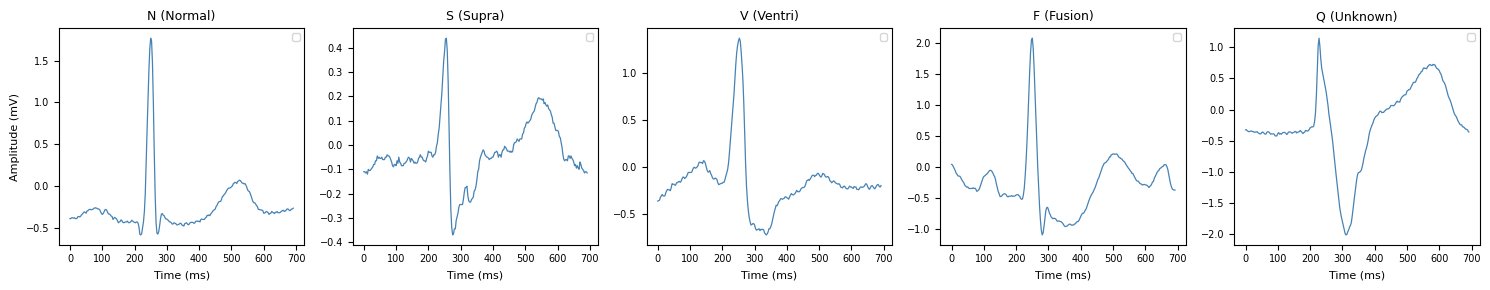
\includegraphics[width=\linewidth]{images/04_examples}
    \caption[MIT-BIH Examples]{MIT-BIH examples for each class.}
    \label{fig:04_examples}
\end{figure}

\subsection{Preprocessing}

Since the MIT-BIH dataset is sufficiently cleaned, little preprocessing was needed.
We have split each of the recordings into individual beats of length $250$, each beat was centered around its annotated peak.
Then a per-beat (per-sample) z-score transformation was applied to ensure each beat has a mean of 0 and a standard deviation of 1.

\begin{align}
    Z = \frac{X - \overline{X}}{\mu}
\end{align}

\begin{center}
    \small Z-score transformation of a variable $X$
\end{center}


\section{Methodology}\label{sec:04_methodology}

In order for the experiments to produce models that are generalizable - perform well on new, unseen data, we must first describe the methodology used for training, evaluation and selection of these models.
The experiments should also be replicable, therefore we use RNG seeding and document all the relevant parameters and configurations for each model.

\subsection{Metric definition}

Since the experiments will be focused on multi-class classification, It is necessary to define the relevant metrics.

\bigskip

\noindent First we define per-class TP, FP, TN, FN as:

\begin{table}[H]
    \centering
    \scriptsize
    \renewcommand{\arraystretch}{1.1}

    \begin{tabularx}{\textwidth}{X c}
        \toprule
        \textbf{Metric} & \textbf{Definition} \tabularnewline \midrule
        $\mathrm{TP}_c$ & \# of instances of class $c$ that were classified as class $c$ \tabularnewline
        $\mathrm{FP}_c$ & \# of instances of classes other than $c$ that were classified as class $c$ \tabularnewline
        $\mathrm{TN}_c$ & \# of instances of classes other than $c$ that were classified as class other than $c$ \tabularnewline
        $\mathrm{FN}_c$ & \# of instances of class $c$ that were classified as class other than $c$ \tabularnewline
        \bottomrule
    \end{tabularx}

    \caption[TP, FP, TN, FN definition]{TP, FP, TN, FN definition.}
    \label{tab:04_tp_fp_tn_fn}
\end{table}

\FloatBarrier

Then we define per-class Precision, Recall and F1-score as:

        {\setlength{\jot}{1em}
\begin{align}
    \mathrm{Precision}_c &= \frac{\mathrm{TP}_c}{\mathrm{TP}_c + \mathrm{FP}_c} \\
    \mathrm{Recall}_c &= \frac{\mathrm{TP}_c}{\mathrm{TP}_c + \mathrm{FN}_c} \\
    \mathrm{F1}_c &= 2 \cdot \frac{\mathrm{Precision}_c \cdot \mathrm{Recall}_c}{\mathrm{Precision}_c + \mathrm{Recall}_c}
\end{align}
}

\begin{center}
    \small Per-class metrics
\end{center}

\bigskip

\noindent We then further define Macro and Weighted Precision, Recall and Macro F1-score (Macro F1) as arithmetic and weighted means of per-class metrics respectively:

        {\setlength{\jot}{1em}
\begin{align}
    \mathrm{Macro Precision} &= \frac{1}{C} \sum^{C}{\mathrm{Precision}_c} \\
    \mathrm{Macro Recall} &= \frac{1}{C} \sum^{C}{\mathrm{Recall}_c} \\
    \mathrm{Macro \, F1} &=  \frac{1}{C} \sum^{C}{\mathrm{F1}_c}
\end{align}

\begin{center}
    \small Macro metrics
\end{center}

\begin{align}
    \mathrm{Weighted Precision} &=  \frac{\sum^{C}{w_c \cdot \mathrm{Precision}_c}}{\sum^{C}{w_c}} \\
    \mathrm{Weighted Recall} &=  \frac{\sum^{C}{w_c \cdot \mathrm{Recall}_c}}{\sum^{C}{w_c}} \\
    \mathrm{Weighted F1} &= \frac{\sum^{C}{w_c \cdot \mathrm{F1}_c}}{\sum^{C}{w_c}}
\end{align}
}

\begin{center}
    \small Weighted metrics
\end{center}

Where $C$ is the number of classes and $w_c$ the number of instances of the class~$c$.

\subsection{Model evaluation}

We adopt the standard \textbf{train}/\textbf{validation}/\textbf{test} protocol for model development and evaluation.
Specifically, the dataset is partitioned into three subsets: \textbf{train}, \textbf{val} and \textbf{test}.

We don't take the individual recordings into account, this allows different beats from one recording to end up in different subsets.
While this approach wouldn't be ideal for real world applications, many other authors use it in their works\parencite{Hu2022, ECGformer}, and it allows us to compare our results to theirs.

\textbf{Model training} is then performed exclusively on the \textbf{train} subset while performance is evaluated\footnote{Evaluation refers to the computation of metrics.} on the \textbf{val} subset after each \textbf{epoch}\footnote{One complete pass over the \textbf{train} subset during training.}.
Based on these validation results, we select the best model \textbf{checkpoint}\footnote{The state of the model after \(n\) epochs.}, primarily according to a chosen performance metric and the discrepancy between \textbf{train} and \textbf{val} performance (large gap typically indicates overfitting).

The selected final checkpoint is then evaluated on the \textbf{test} subset, which serves as an approximation of performance on previously unseen data.
Throughout preprocessing, special care must be taken to prevent information leakage into the \textbf{test} subset.

As a main performance metric for selection of our classifier models we've decided to choose Macro F1.
While we've previously discussed the importance of Recall in medical applications Macro F1 is used as a main metric in many other publications \parencite{Hu2022} and will allow us to effectively compare our models against other solutions.
At the same time, Macro F1 still places strong emphasis on Recall through its harmonic formulation, making it aligned with our objective of accurately identifying important minority classes.


\section{Experiments}

We've performed multiple experiments with various transformer-based classifiers and different configurations / parameters for each model.
For clarity, we show only the configurations that performed well or were otherwise interesting.

\subsection{Weighted Loss}\label{subsec:04-weighted-loss}

Due to the imbalance of classes in the dataset a commonly used \textbf{Cross-Entropy Loss} ($L_{\mathrm{CE}}$) performed badly on the data.
Because of this, we've decided to adopt \textbf{Weighted Cross-Entropy Loss} ($L_{\mathrm{WCE}}$) which mitigates the imbalance by taking the class weights into account.

\begin{align}
    L_{\mathrm{CE}}(Y, \hat{p}) &= - \sum_{c=1}^{C} y_c \log \hat{p}_c \label{eq:04-cross-entropy} \\
    L_{\mathrm{WCE}}(Y, \hat{p}) &= - \sum_{c=1}^{C} \alpha_c \, y_c \log \hat{p}_c \label{eq:04-weighted-cross-entropy}
\end{align}

\subsection{Base Transformer}\label{subsec:04-base-transformer}

As the first configuration, we trained an encoder-only transformer model from scratch.

\subsubsection{Architecture}

\begin{enumerate}
    \item The ECG signal of length \textbf{250} was tokenized into \textbf{25} non-overlapping patches of size \textbf{10}.
    \item These tokens are then projected into dimension $d_{\mathrm{model}}$ using a linear layer, positional embeddings are also added.
    \item A learnable classification (CLS) token is then appended and the entire sequence is put through the encoder blocks.
    \item Then, the last token is extracted (last token pooling) and using a linear classifier layer, probability logits are obtained.
\end{enumerate}

The following model configuration was used:

\FloatBarrier

\begin{table}[H]
    \centering
    \small
    \renewcommand{\arraystretch}{1.1}

    \begin{tabularx}{0.6\textwidth}{X c}
        \toprule
        \textbf{Parameter} & \textbf{Value} \tabularnewline
        \midrule
        $d_{\mathrm{model}}$ & $256$ \tabularnewline
        $d_{\mathrm{ff}}$    & $1024$ \tabularnewline
        $n_{\mathrm{head}}$  & $8$ \tabularnewline
        $n_{\mathrm{layer}}$ & $8$ \tabularnewline
        Activation Function & ReLU \tabularnewline
        \bottomrule
    \end{tabularx}

    \caption[Base Transformer Configuration]{Base Transformer Configuration.}
    \label{tab:04_base_transformer_configuration}
\end{table}

\FloatBarrier

\subsubsection{Training}

The training took around 5 minutes, the following parameters were used:

\begin{table}[H]
    \centering
    \small
    \renewcommand{\arraystretch}{1.1}

    \begin{tabularx}{0.6\textwidth}{X c}
        \toprule
        \textbf{Parameter} & \textbf{Value} \tabularnewline
        \midrule
        Epochs        & $100$ \tabularnewline
        Learning Rate & $5 \times 10^{-5}$ \tabularnewline
        Batch Size    & $128$ \tabularnewline
        Dropout       & $0.15$ \tabularnewline
        Loss          & WeightedLoss \tabularnewline
        Optimizer     & AdamW \tabularnewline
        Weight Decay  & $1 \times 10^{-2}$ \tabularnewline
        \bottomrule
    \end{tabularx}

    \caption[Base Transformer Training Parameters]{Training Parameters.}
    \label{tab:04_base_transformer_training}
\end{table}

\FloatBarrier

Previous work by \textcite{Hu2022, ECGformer} was used as the basis for the used hyperparameters.

Training loss continued to decrease over the training, the training and validation loss diverged at around epoch $20$ and validation loss started increasing at around epoch $40$.
Validation Macro F1 reached the best value at epoch $53$ and stagnated afterward.

\begin{figure}[!htbp]
    \centering
    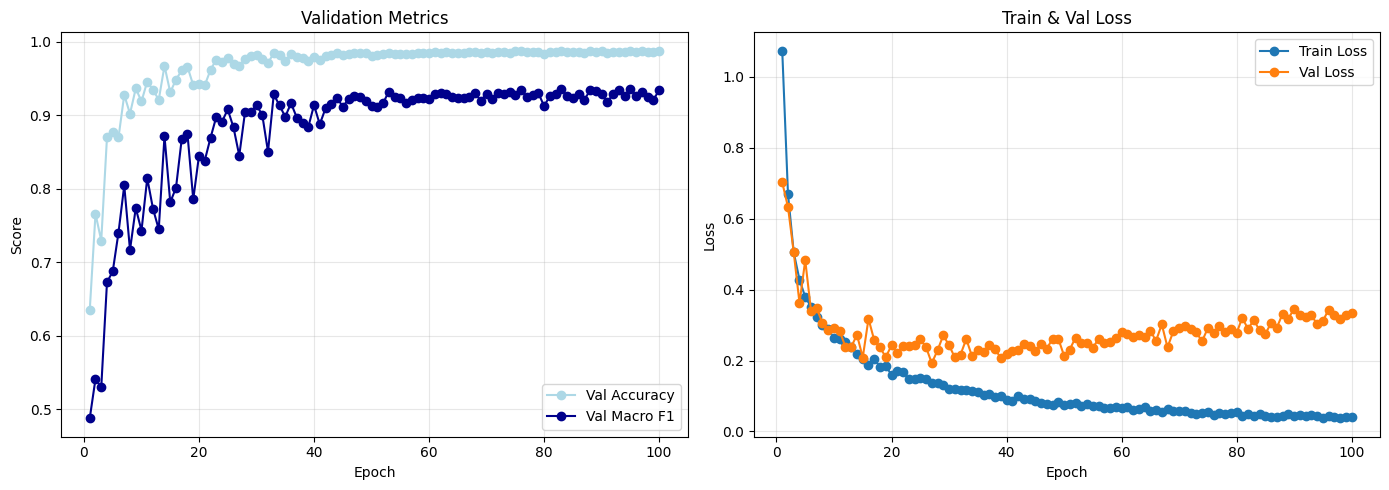
\includegraphics[width=0.9\linewidth]{images/04/base_transformer_training_curves}
    \caption[Base Transformer Training Curves]{Training Curves.}
    \label{fig:04_base_transformer_training_curves}
\end{figure}

\FloatBarrier

\subsubsection{Evaluation}


Checkpoint at epoch $53$ was chosen for detailed evaluation on the \textbf{val} set due to its best Macro F1.

\begin{table}[H]
    \centering
    \footnotesize
    \renewcommand{\arraystretch}{1.1}

    \begin{minipage}[t]{0.32\textwidth}
        \centering
        \begin{tabularx}{\textwidth}{X c}
            \toprule
            \textbf{Metric} & \textbf{Score} \tabularnewline
            \midrule
            Accuracy    & 0.9853 \tabularnewline
            Macro F1    & 0.9320 \tabularnewline
            Weighted F1 & 0.9856 \tabularnewline
            \bottomrule
        \end{tabularx}
    \end{minipage}
    \hfill
    \begin{minipage}[t]{0.64\textwidth}
        \centering
        \footnotesize
        \begin{tabularx}{\textwidth}{X c c c c}
            \toprule
            \textbf{Class} & \textbf{Precision} & \textbf{Recall} & \textbf{F1-score} & \textbf{Support} \tabularnewline
            \midrule
            N & 1.00 & 0.99 & 0.99 & 19025 \tabularnewline
            S & 0.80 & 0.91 & 0.85 & 584   \tabularnewline
            V & 0.95 & 0.98 & 0.97 & 1519  \tabularnewline
            F & 0.85 & 0.88 & 0.86 & 169   \tabularnewline
            Q & 0.99 & 1.00 & 0.99 & 1688  \tabularnewline
            \bottomrule
        \end{tabularx}
    \end{minipage}

    \caption[Base Transformer Evaluation Metrics]{Evaluation Metrics.}
    \label{tab:04_base_transformer_evaluation_metrics}
\end{table}

\FloatBarrier

\begin{figure}[!htbp]
    \centering
    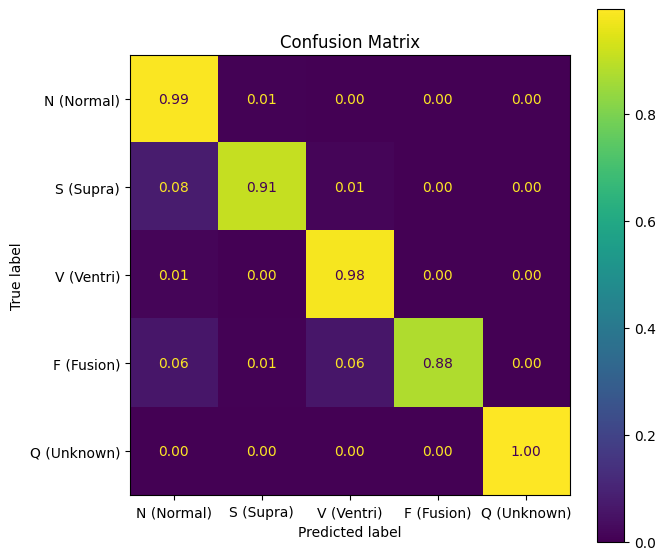
\includegraphics[width=0.6\linewidth]{images/04/base_transformer_confusion_matrix}
    \caption[Base Transformer Confusion Matrix]{Confusion Matrix.}
    \label{fig:04_base_transformer_confusion_matrix}
\end{figure}

\FloatBarrier

The baseline model performed excellently at $\mathrm{Macro \, F1} = 0.93$.
Additionally, we can see that the model achieved per-class performance at rate proportional to the class's support with classes \textbf{S} and \textbf{F} having the worst scores.

\subsection{Qwen2.5 0.5B fine-tune}

For the next experiment we've performed a LoRA fine-tune of pretrained a Qwen2.5 0.5B\footnote{https://huggingface.co/Qwen/Qwen2.5-0.5B} \parencite{qwen2025} LLM\@.
The size of 0.5B (500 million parameters) made it small enough to effectively fine-tune on available hardware (AMD Radeon RX 9070 GPU).

\subsubsection{Architecture}

We used the same approach for tokenization and embedding as in the first experiment, entirely bypassing the original tokenizer and embedding layer.
A learnable CLS token with the classification layer was also implemented, resulting in nearly identical architecture to the first experiment, only difference being the pretrained transformer stack.

\begin{table}[H]
    \centering
    \small
    \renewcommand{\arraystretch}{1.1}

    \begin{tabularx}{0.6\textwidth}{X c}
        \toprule
        \textbf{Parameter} & \textbf{Value} \tabularnewline
        \midrule
        $d_{\mathrm{model}}$ & $896$ \tabularnewline
        $d_{\mathrm{ff}}$    & $4864$ \tabularnewline
        $n_{\mathrm{head}}$  & $16$ \tabularnewline
        $n_{\mathrm{layer}}$ & $24$ \tabularnewline
        Activation Function & SwiGLU \tabularnewline
        \bottomrule
    \end{tabularx}

    \caption[Qwen 2.5 0.5B Configuration]{Configuration.}
    \label{tab:04_qwen2.5_0.5b_configuration}
\end{table}

\FloatBarrier

\subsubsection{Training}

The training took around 90 minutes, the following parameters were used:

\begin{table}[H]
    \centering
    \small
    \renewcommand{\arraystretch}{1.1}

    \begin{tabularx}{0.6\textwidth}{X c}
        \toprule
        \textbf{Parameter} & \textbf{Value} \tabularnewline
        \midrule
        Epochs        & $30$ \tabularnewline
        Learning Rate & $5 \times 10^{-5}$ \tabularnewline
        Batch Size    & $128$ \tabularnewline
        Dropout       & $0.15$ \tabularnewline
        Loss          & WeightedLoss \tabularnewline
        Optimizer     & AdamW \tabularnewline
        Weight Decay  & $1 \times 10^{-2}$ \tabularnewline
        LoRA rank     & $8$ \tabularnewline
        LoRA $\alpha$ & $16$ \tabularnewline
        \bottomrule
    \end{tabularx}

    \caption[Qwen 2.5 0.5B Training Parameters]{Training Parameters.}
    \label{tab:04_qwen_2.5_0.5b_training}
\end{table}

\FloatBarrier

The model started converging much faster than in the first experiment, achieving $0.90$ validation Macro F1 in $7$, however after that point at around epoch $10$, the validation loss diverged from the training loss and immediately started increasing

\begin{figure}[!htbp]
    \centering
    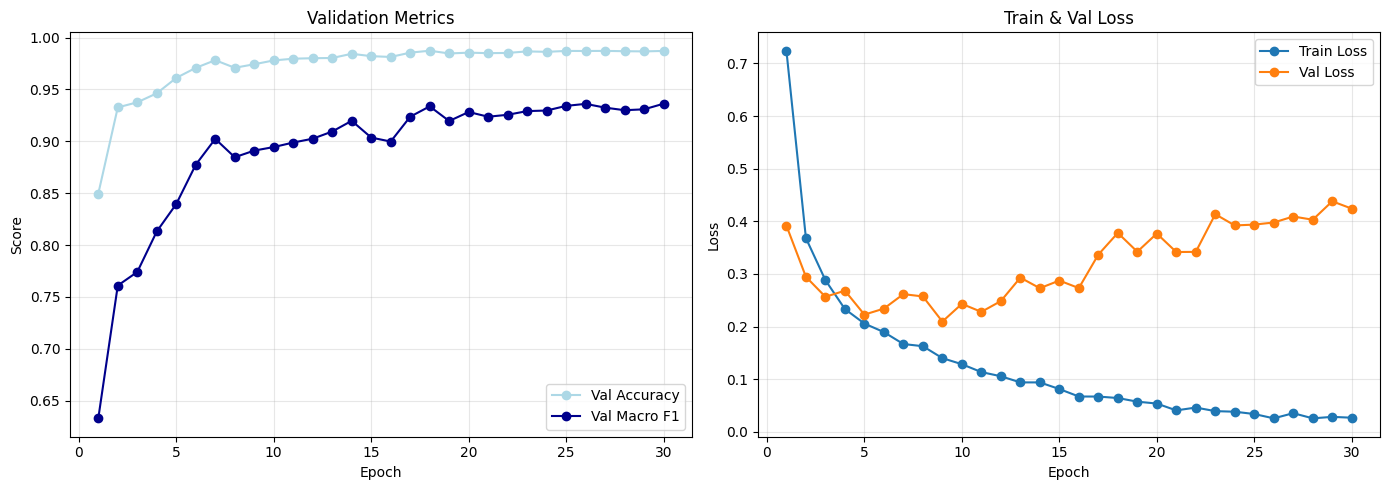
\includegraphics[width=0.9\linewidth]{images/04/llm_training_curves}
    \caption[Qwen 2.5 0.5B Training Metrics]{Training Metrics.}
    \label{fig:04_qwen_2.5_0.5b_training_metric}
\end{figure}

\FloatBarrier

\subsubsection{Evaluation}

Checkpoint at epoch $7$ was chosen for further evaluation on val dataset as the best model due to its best val Macro F1 before divergence and probable overfitting started happening.

\begin{table}[H]
    \centering
    \footnotesize
    \renewcommand{\arraystretch}{1.1}

    \begin{minipage}[t]{0.32\textwidth}
        \centering
        \begin{tabularx}{\textwidth}{X c}
            \toprule
            \textbf{Metric} & \textbf{Score} \tabularnewline
            \midrule
            Accuracy    & 0.9782 \tabularnewline
            Macro F1    & 0.9024 \tabularnewline
            Weighted F1 & 0.9787 \tabularnewline
            \bottomrule
        \end{tabularx}
    \end{minipage}
    \hfill
    \begin{minipage}[t]{0.64\textwidth}
        \centering
        \footnotesize
        \begin{tabularx}{\textwidth}{X c c c c}
            \toprule
            \textbf{Class} & \textbf{Precision} & \textbf{Recall} & \textbf{F1-score} & \textbf{Support} \tabularnewline
            \midrule
            N & 0.99 & 0.98 & 0.99 & 19025 \tabularnewline
            S & 0.73 & 0.86 & 0.79 & 584   \tabularnewline
            V & 0.92 & 0.98 & 0.94 & 1519  \tabularnewline
            F & 0.80 & 0.80 & 0.80 & 169   \tabularnewline
            Q & 0.99 & 0.99 & 0.99 & 1688  \tabularnewline
            \bottomrule
        \end{tabularx}
    \end{minipage}

    \caption[Qwen 2.5 0.5B Evaluation Metrics]{Evaluation Metrics.}
    \label{tab:04_qwen_2.5_0.5b_evaluation_metrics}
\end{table}

\FloatBarrier

\begin{figure}[!htbp]
    \centering
    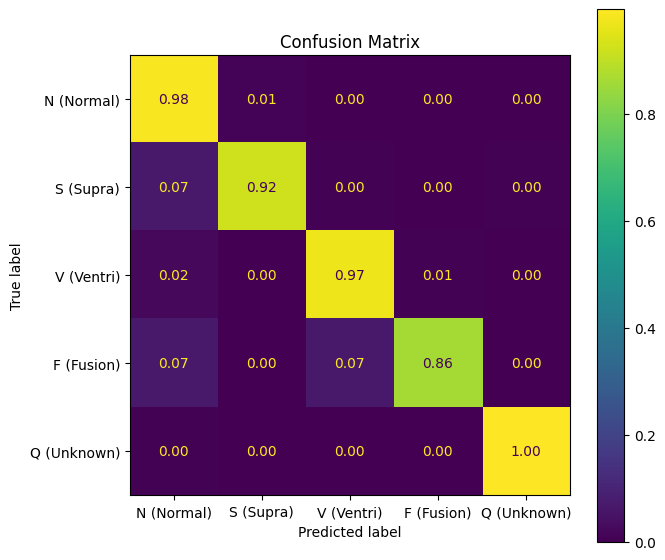
\includegraphics[width=0.6\linewidth]{images/04_qwen_2.5_0.5b_confusion_matrix}
    \caption[Qwen 2.5 0.5B Confusion Matrix]{Confusion Matrix.}
    \label{fig:04_qwen_2.5_0.5b_confusion_matrix}
\end{figure}

\FloatBarrier


\section{Results and Discussion}

The first base transformer outperformed the second LLM fine-tune model and its checkpoint at epoch $53$ was therefore chosen as the model for final evaluation on the \textbf{test} set.

\begin{table}[H]
    \centering
    \footnotesize
    \renewcommand{\arraystretch}{1.1}

    \begin{minipage}[t]{0.32\textwidth}
        \centering
        \begin{tabularx}{\textwidth}{X c}
            \toprule
            \textbf{Metric} & \textbf{Score} \tabularnewline
            \midrule
            Accuracy    & 0.9839 \tabularnewline
            Macro F1    & 0.9253 \tabularnewline
            Weighted F1 & 0.9843 \tabularnewline
            \bottomrule
        \end{tabularx}
    \end{minipage}
    \hfill
    \begin{minipage}[t]{0.64\textwidth}
        \centering
        \footnotesize
        \begin{tabularx}{\textwidth}{X c c c c}
            \toprule
            \textbf{Class} & \textbf{Precision} & \textbf{Recall} & \textbf{F1-score} & \textbf{Support} \tabularnewline
            \midrule
            N & 1.00 & 0.99 & 0.99 & 8154 \tabularnewline
            S & 0.77 & 0.93 & 0.84 & 250  \tabularnewline
            V & 0.94 & 0.97 & 0.96 & 651  \tabularnewline
            F & 0.84 & 0.85 & 0.84 & 72   \tabularnewline
            Q & 0.99 & 0.99 & 0.99 & 724  \tabularnewline
            \bottomrule
        \end{tabularx}
    \end{minipage}

    \caption[Final Model Evaluation Metrics]{Final Model Evaluation Metrics.}
    \label{tab:04_final_model_evaluation_metrics}
\end{table}

\FloatBarrier

\begin{figure}[!htbp]
    \centering
    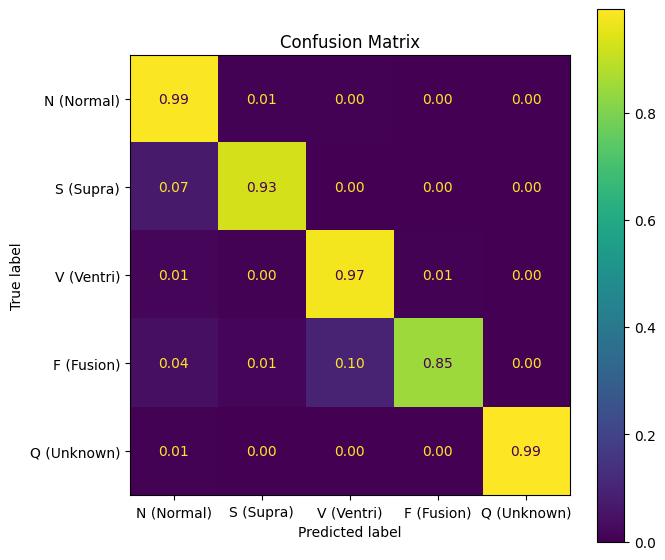
\includegraphics[width=0.6\linewidth]{images/04/test_confusion_matrix}
    \caption[Final Model Confusion Matrix]{Final Model Confusion Matrix.}
    \label{fig:final_model_confusion_matrix}
\end{figure}

\FloatBarrier

The final model performed only slightly worse on the unseen test data ($\Delta \mathrm{Macro \, F1} \leq 0.01$) and has shown that transformer-based models are suitable for the classification of time series.

The LLM fine-tune solution still performed surprisingly well and shows that even older and very small LLMs can achieve performance comparable to specialized models.
With more modern and larger models (like Qwen3.6 series) the performance might've been even better, however such experiments are costly due to the immense computational costs of fine-tuning (larger models require clusters of high-end GPUs even for a (Q)LoRA fine-tune).

\subsection{Comparison with Other Work}

Additionally, we provide a comparison of our models with the work of other authors.

\begin{table}[ht]
    \centering
    \small
    \renewcommand{\arraystretch}{1.1}
    \begin{tabularx}{\textwidth}{Xcccc}
        \toprule
        \textbf{Model} & \textbf{Macro F1 Score} & \textbf{Accuracy} & \textbf{Method} \tabularnewline \midrule
        \cite{Hu2022} ($\alpha$) & 0.94 & 0.99 & Transformer \tabularnewline
        Base Transformer & 0.93 & 0.98 & Transformer \tabularnewline
        Qwen 2.5 0.5B fine-tune & 0.90 & 0.98 & LoRA fine-tune \tabularnewline
        \cite{Mousavi2021} & 0.87 & 0.98 & ELP + CNN \tabularnewline
        \cite{ECGformer} & 0.86 & 0.98 & Transformer \tabularnewline
        \bottomrule
    \end{tabularx}
    \caption[Comparison of Results]{Comparison of different models, ordered by Macro F1 Score.}
    \label{tab:04_comparison_of_results}
\end{table}









